%% For double-blind review submission, w/o CCS and ACM Reference (max submission space)
\documentclass[sigplan,10pt,review,anonymous]{acmart}\settopmatter{printfolios=true,printccs=false,printacmref=false}
%% For double-blind review submission, w/ CCS and ACM Reference
%\documentclass[sigplan,10pt,review,anonymous]{acmart}\settopmatter{printfolios=true}
%% For single-blind review submission, w/o CCS and ACM Reference (max submission space)
%\documentclass[sigplan,10pt,review]{acmart}\settopmatter{printfolios=true,printccs=false,printacmref=false}
%% For single-blind review submission, w/ CCS and ACM Reference
%\documentclass[sigplan,10pt,review]{acmart}\settopmatter{printfolios=true}
%% For final camera-ready submission, w/ required CCS and ACM Reference
%\documentclass[sigplan,10pt]{acmart}\settopmatter{}


%% Conference information
%% Supplied to authors by publisher for camera-ready submission;
%% use defaults for review submission.
\acmConference[REBLS'18]{ACM SIGPLAN Workshop on Reactive and Event-Based Languages and Systems}{November 04, 2018}{Boston, MA, USA}
\acmYear{2018}
\acmISBN{} % \acmISBN{978-x-xxxx-xxxx-x/YY/MM}
\acmDOI{} % \acmDOI{10.1145/nnnnnnn.nnnnnnn}
\startPage{1}

%% Copyright information
%% Supplied to authors (based on authors' rights management selection;
%% see authors.acm.org) by publisher for camera-ready submission;
%% use 'none' for review submission.
\setcopyright{none}
%\setcopyright{acmcopyright}
%\setcopyright{acmlicensed}
%\setcopyright{rightsretained}
%\copyrightyear{2017}           %% If different from \acmYear

%% Bibliography style
\bibliographystyle{ACM-Reference-Format}
%% Citation style
%\citestyle{acmauthoryear}  %% For author/year citations
%\citestyle{acmnumeric}     %% For numeric citations
%\setcitestyle{nosort}      %% With 'acmnumeric', to disable automatic
                            %% sorting of references within a single citation;
                            %% e.g., \cite{Smith99,Carpenter05,Baker12}
                            %% rendered as [14,5,2] rather than [2,5,14].
%\setcitesyle{nocompress}   %% With 'acmnumeric', to disable automatic
                            %% compression of sequential references within a
                            %% single citation;
                            %% e.g., \cite{Baker12,Baker14,Baker16}
                            %% rendered as [2,3,4] rather than [2-4].


%%%%%%%%%%%%%%%%%%%%%%%%%%%%%%%%%%%%%%%%%%%%%%%%%%%%%%%%%%%%%%%%%%%%%%
%% Note: Authors migrating a paper from traditional SIGPLAN
%% proceedings format to PACMPL format must update the
%% '\documentclass' and topmatter commands above; see
%% 'acmart-pacmpl-template.tex'.
%%%%%%%%%%%%%%%%%%%%%%%%%%%%%%%%%%%%%%%%%%%%%%%%%%%%%%%%%%%%%%%%%%%%%%


%% Some recommended packages.
\usepackage{booktabs}   %% For formal tables:
                        %% http://ctan.org/pkg/booktabs
\usepackage{subcaption} %% For complex figures with subfigures/subcaptions
                        %% http://ctan.org/pkg/subcaption

\usepackage{xspace}
\newcommand{\CEU}{\textsc{C\'{e}u}\xspace}

\newcommand{\code}[1] {{\small{\texttt{#1}}}}

\usepackage{listings}
\lstdefinelanguage{ceu}{%
  language=C,
  morekeywords={%
    @const, @pure, @safe, NEVER, FOREVER, PAR, PROC, SIGNAL, abort, and,
    await, bool, call, class, data, define, deterministic, do, each, else,
    emit, end, escape, event, every, finalize, hor, implementation, in,
    input, interface, loop, min, native, new, nohold, not, or, output, par,
    pool, pure, return, s, h, ms, signal, spawn, tag, then, this, traverse, until,
    code, public, private,
    var, watching, when, with},
}
\lstset{
  literate={~} {$\sim$}{1},
  basicstyle=\footnotesize\ttfamily,
  captionpos=b,
  columns=flexible,
  commentstyle=\footnotesize\itshape,
  escapeinside={||},
  frame=tb,
  keepspaces=true,
  keywordstyle=\bfseries,
  language=ceu,
  numbersep=4pt,
  numberstyle=\tiny,
  %xleftmargin=0.5cm,
  %xrightmargin=0.5cm,
  %upquote=true,
}

\usepackage{tikz}
\usetikzlibrary{
  arrows,
  arrows.meta,
  calc,
  decorations.pathreplacing,
  decorations.text,
  math,
  positioning,
  shapes,
}

\begin{document}

%% Title information
\title{Where Do Events Come From?}
\subtitle{Reactive and Energy-Efficient Programming From The Ground Up}

%% Author information
%% Contents and number of authors suppressed with 'anonymous'.
%% Each author should be introduced by \author, followed by
%% \authornote (optional), \orcid (optional), \affiliation, and
%% \email.
%% An author may have multiple affiliations and/or emails; repeat the
%% appropriate command.
%% Many elements are not rendered, but should be provided for metadata
%% extraction tools.

%% Author with single affiliation.
\author{First1 Last1}
\authornote{with author1 note}          %% \authornote is optional;
                                        %% can be repeated if necessary
\orcid{nnnn-nnnn-nnnn-nnnn}             %% \orcid is optional
\affiliation{
  \position{Position1}
  \department{Department1}              %% \department is recommended
  \institution{Institution1}            %% \institution is required
  \streetaddress{Street1 Address1}
  \city{City1}
  \state{State1}
  \postcode{Post-Code1}
  \country{Country1}                    %% \country is recommended
}
\email{first1.last1@inst1.edu}          %% \email is recommended

%% Author with two affiliations and emails.
\author{First2 Last2}
\authornote{with author2 note}          %% \authornote is optional;
                                        %% can be repeated if necessary
\orcid{nnnn-nnnn-nnnn-nnnn}             %% \orcid is optional
\affiliation{
  \position{Position2a}
  \department{Department2a}             %% \department is recommended
  \institution{Institution2a}           %% \institution is required
  \streetaddress{Street2a Address2a}
  \city{City2a}
  \state{State2a}
  \postcode{Post-Code2a}
  \country{Country2a}                   %% \country is recommended
}
\email{first2.last2@inst2a.com}         %% \email is recommended
\affiliation{
  \position{Position2b}
  \department{Department2b}             %% \department is recommended
  \institution{Institution2b}           %% \institution is required
  \streetaddress{Street3b Address2b}
  \city{City2b}
  \state{State2b}
  \postcode{Post-Code2b}
  \country{Country2b}                   %% \country is recommended
}
\email{first2.last2@inst2b.org}         %% \email is recommended


%% Abstract
%% Note: \begin{abstract}...\end{abstract} environment must come
%% before \maketitle command

\begin{abstract}
In reactive and event-based systems, execution is guided by an external
environment that generates inputs to the application and consumes outputs from
it.
Reactive languages provide dedicated syntax and semantics to deal with events
and greatly simplify the programming experience in this domain.
%
Nevertheless, the environment is typically prefabricated in a host language and
the very central concept of events is implemented externally to the reactive
language.
%
In this work, we propose an interrupt handler primitive for a reactive language
targeting embedded systems in order to take control of the whole event loop:
from a sensor input source and back to an actuator output.
%
We propose the new asynchronous primitive in the context of the synchronous
language \CEU and discuss how they synergize to avoid race conditions at
compile time, support lexically-scoped drivers, and provide automatic standby
for applications.
%and hot swapping of device drivers
\end{abstract}

%% 2012 ACM Computing Classification System (CSS) concepts
%% Generate at 'http://dl.acm.org/ccs/ccs.cfm'.
\begin{CCSXML}
<ccs2012>
<concept>
<concept_id>10011007.10011006.10011008</concept_id>
<concept_desc>Software and its engineering~General programming languages</concept_desc>
<concept_significance>500</concept_significance>
</concept>
<concept>
<concept_id>10003456.10003457.10003521.10003525</concept_id>
<concept_desc>Social and professional topics~History of programming languages</concept_desc>
<concept_significance>300</concept_significance>
</concept>
</ccs2012>
\end{CCSXML}

\ccsdesc[500]{Software and its engineering~General programming languages}
\ccsdesc[300]{Social and professional topics~History of programming languages}
%% End of generated code


%% Keywords
%% comma separated list
\keywords{
    interrupt service routines,
    reactive programming,
    sleep modes,
    standby,
    synchronous/asynchronous execution
}

\maketitle

\section{Introduction}

Reactive applications interact continuously and in real time with the external
world through hardware peripherals such as sensors and actuators (e.g.,
buttons, displays, timers, etc.).
%
These interactions are typically represented in software as input events
flowing from the peripherals to the application and as output events flowing
from the application to the peripherals.
%
As illustrated in Figure~\ref{fig.env}, peripherals can be encapsulated as a
single component, \emph{the environment}, which connects with the application
in an event loop:
the application sits idle until the environment awakes it on the occurrence of
an input;
the application reacts to the input and generates back one or more outputs
which affect the environment;
the application becomes idle and the loop restarts.

\begin{figure}
\centering
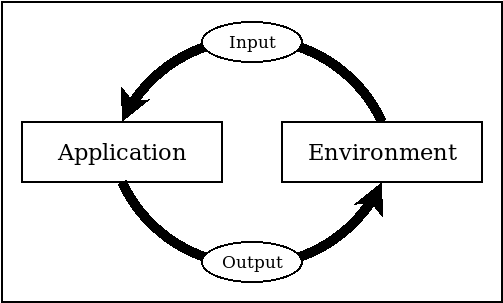
\includegraphics[width=\linewidth]{loop}
\caption{ Event loop in reactive systems.
          The environment controls the application through input \& output
          events.
\label{fig.env}
}
\end{figure}

The environment is typically implemented in a host language (e.g., C) and
controls the main event loop, invoking entry points into the reactive language
runtime on the occurrence of inputs, and also receiving output calls from it,
both through a documented API.
%
As examples, Esterel~\cite{esterel.ieee91} relies on C for passing events
between the environment and the running program~\cite{esterel.book.compiling},
while Elm~\cite{frp.elm} uses the concept of \emph{ports}, which allows sending
out values to JavaScript as commands and listening for values as
subscriptions~\cite{frp.elm.ports}.

The event-based interface between the application and the environment is
arguably inevitable and also happens at the appropriate layer, since it
connects the application with the operating system resources through a
non-invasive API.
%
However, this separation reveals the environment as a rigid system component
that evolves in separate from the application.
%
It also requires two languages and the programmer has to deal with multiple
syntaxes, incompatible type systems, and different address spaces.
%
Furthermore, in the context of embedded systems, a proper host OS may even be
absent or lacking enough device drivers, which requires more low-level
intervention from the application.

In this work, we propose interrupt service routines (ISRs) as an asynchronous
primitive for the synchronous language \CEU~\cite{ceu.sensys13}.
ISRs empower reactive applications to also implement their own device drivers
and self-generate inputs, bypassing the need for a host environment.
%
\CEU targets resource-constrained architectures, such as Arduino-compatible
microcontrollers, in which applications run in the bare metal, without
operating system support.
In this context, device drivers are typically libraries compiled together with
the main program.

The lack of an OS opens an opportunity to explore a tighter integration between
the application and its device drivers at the language level, resulting in an
overall simplicity and tractability of the system.
%
In particular, \CEU is already amenable to a simple static analysis to detect
race conditions which we extended in this work to also encompass ISRs.
Applications can share data buffers with drivers to avoid unnecessary copying,
with some static guarantee that no data races will occur.
%
\CEU also provides a lexical finalization mechanism that we adopt in drivers to
properly disable interrupts and turn off peripherals completely.
For instance, we can delimit the scope of a driver similarly to a
lexically-scoped variables.
%
Finally, the synchronous semantics of \CEU enforces that applications react
to inputs in bounded time and remain in idle states susceptible to standby.
With the help of drivers and a power manager, we can put the microcontroller to
sleep automatically at optimal sleeping modes after each input reaction.

We implemented an extensible runtime that exposes hooks for the interrupts and
power manager, which we validated in two microcontrollers: an
\emph{8-bit AVR/ATmega} and a \emph{32-bit ARM/Cortex-M0}.
%
We also implemented drivers for a variety of peripherals, such as GPIO, A/D
converter, USART, SPI, and nRF24L01 transceiver.
%
The applications built on top of these drivers show significant energy savings
due to automatic standby.

TODO: weakness

\begin{comment}
% Esterel
https://books.google.com.br/books?id=O5zi14i0KP4C&pg=PA31&lpg=PA31&dq=esterel+external+signal+api&source=bl&ots=43EBAqIkSJ&sig=npYylZteOmZAqv4f7SXAtJO9xr8&hl=en&sa=X&ved=0ahUKEwjFlf7-3p_cAhWPrVkKHXsFDWgQ6AEIUjAG#v=onepage&q=esterel%20external%20signal%20api&f=false
Esterel relies on general-purpose languages such as C or C++ in two ways.       
First, for portability, most Esterel compilers generate C instead of            
assembly or some other executable representation.                               
Such generated code provides an interface for passing events between the        
environment and the running program.                                            
Second, Esterel allows the use of data types and functions defined externally   
(e.g., in C) to be used within an Esterel program.                              

% Elm
https://guide.elm-lang.org/interop/javascript.html
Okay, in Elm, any communication with JavaScript goes through a port. Think of
it like a hole in the side of your Elm program where you can send values in and
out. These work exactly like the commands and subscriptions from the
Architecture section. Sending values out to JS is a command. Listening for
values coming in from JS is a subscription. Pretty neat!
\end{comment}

\section{\CEU: Structured Synchronous Reactive Programming}
\label{sec.ceu}

\CEU~\cite{ceu.sensys13} is a Esterel-based~\cite{ceu.tecs17} reactive
programming language targeting resource-constrained embedded systems, with the
characteristics that follow:
%
\begin{description}
\item [Reactive:] code only executes in reactions to events and is idle most of
    the time.
\item [Structured:] programs use lexically-scoped structured control
    mechanisms such as \code{spawn} and \code{await} (to create and suspend
    lines of execution).
\item [Synchronous:] reactions run atomically and to completion on each line of
    execution, i.e., there's no implicit preemption or real parallelism.
\end{description}

Structured reactive programming lets developers write code in direct style,
recovering from the inversion of control imposed by event-driven
execution~\cite{rp.deprecating,rp.rescala,sync_async.cooperative}.

\begin{lstlisting}[
  xleftmargin=1em,
  numbers=left,
  basicstyle=\ttfamily\small,
  float=h,
  caption={A \CEU program that toggles the state of the LED whenever a radio
           packet is received, terminating on a button press, always with the
           LED off.},
  label={lst.ceu},
]
output high/low LED;
input  high/low BUTTON;
input  Packet   RADIO_RECV;
par/or do
    var high/low v = await BUTTON until (v==low);
with
    finalize with
        emit LED(low);
    end
    loop do
        emit LED(high);
        await RADIO_RECV;
        emit LED(low);
        await RADIO_RECV;
    end
end
\end{lstlisting}

Listing~\ref{lst.ceu} illustrates the main characteristics of \CEU, namely
event-driven I/O, lexically-scoped compositions, and synchronous execution.
%
The program toggles the state of the LED whenever a radio packet is received,
terminating on a button press, always with the LED off.
%
The program first declares the \code{LED} output, and the \code{BUTTON} and
\code{RADIO\_RECV} input events (ln~1--3).
The declarations include a payload type, i.e., each event occurrence carries
a value of that type (\code{high/low} is a boolean type).
%
Then, the program uses a \code{par/or} composition (ln~4--16) to run two lines
of execution, aka \emph{trails}, in parallel:
a single-statement trail that waits for a button press before terminating
(ln~5), and an endless loop that toggles the LED on and off whenever a radio
packet is received (ln~10--15).
The \code{finalize} clause (ln~7--9) ensures that, no matter how its enclosing
trail terminates (e.g., from a button press), the LED will be unconditionally
turned off~(ln~8).

All communication between the application and the environment is done through
the \code{await} and \code{emit} primitives, which awaits an input event and
generates an output event, respectively.

The \code{par/or}, which stands for \emph{parallel-or}, is a lexical
composition that terminates as soon as one of the trails terminates, but which
also automatically aborts and finalizes the other trail(s).
%
In the example, when the button is pressed (ln~5), not only the toggling loop
will be aborted (ln~10--15), but the \code{finalize} clause will turn the LED
off unconditionally (ln~8), since its enclosing block goes out of scope.
%
The \code{par/or} is regarded as an \emph{orthogonal preemption
primitive}~\cite{esterel.preemption} because the trails need not to be tweaked
in order to affect each other.

The synchronous execution model of \CEU dictates that reactions to input events
are atomic and that incoming events are never lost.
%
The event loop in Figure~\ref{fig.env} suggests this behavior since the
environment can only generate a new input after the application yields control
and closes the loop.
%
In Listing~\ref{lst.ceu}, even if two packets arrive simultaneously in the
environment, the synchronous model ensures atomicity and responsiveness in the
application:
    the first \code{await} awakes and turns the LED off atomically
    (ln~12--13);
    and the second \code{await} will awake in sequence (ln~14).
%
%Note that if multiple trails in parallel await the same input, they will all
%awake from it during the same reaction.
%In this case, \CEU dictates that each trail executes atomically, one after the
%other, in lexical order.
%This rule prevents race conditions for trails in parallel.

Figure~\ref{fig.ticks} illustrates the synchronous execution model of \CEU.
%
The continuous timeline (representing the environment) shows
``physical timestamps'' for the event occurrences (e.g., event~\code{C}
occurs exactly at 17ms521us).
%
The discrete timeline in the application shows how the same occurring events
fit in the logical notion of time of \CEU.
%
The boot reaction \code{boot-0} happens before any input and starts the
program.
%
Event~\code{A} ``physically'' occurs during \code{boot-0} but, because time
is discrete, its corresponding reaction only executes at logical
instant~\code{A-1}.
%
Similarly, event~\code{B} occurs during~\code{A-1} and its reaction is
postponed to execute at~\code{B-2}.
%
Event~\code{C} also occurs during~\code{A-1} but its reaction must also wait
for~\code{B-2} to execute at~\code{C-3}.
%
Finally, event~\code{D} occurs during an idle period and can start immediately
at \code{D-4}.
%
%Finally, two instances of event~\code{E} occur during~\code{D-4}; they are
%handled in the subsequent reactions~\code{E-5} and~\code{E-6}.

\begingroup
\begin{figure}[t]
\centering
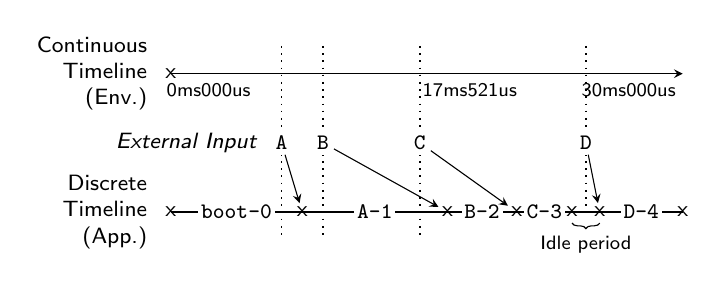
\begin{tikzpicture}[x=1em,y=1em,
  font=\footnotesize\sffamily,>=stealth,
  time/.style={font=\scriptsize\sffamily},
  cross/.style={inner sep=0pt,outer sep=0pt},
  evt/.style={fill=white,inner sep=1.85pt,outer sep=0pt},
  rng/.style={fill=white,inner sep=1pt,outer sep=0pt,
    font=\ttfamily\footnotesize}]
  \draw[->]
  (0,0)
    node[align=right,anchor=east,xshift=-.5em]
        {Continuous\\Timeline\\(Env.)}
    node[anchor=north west,xshift=-.5em,time]
        {0ms000us}
    node[anchor=north west,xshift=8.75em,time]
        {17ms521us}
  -- (18.5,0)
    node[anchor=north east,xshift=.1em,time]
        {30ms000us};
  \node[cross] at (0,0){x};
  %%
  \coordinate(Ext) at ($(0,0)!.5!(0,-5)$);
  \coordinate(A) at (Ext-|4,0);
  \coordinate(B) at (Ext-|5.5,0);
  \coordinate(C) at (Ext-|9,0);
  \coordinate(D) at (Ext-|15,0);
  %%
  \draw[semithick,dotted] (0,1-|A) -- (0,-6-|A);
  \draw[semithick,dotted] (0,1-|B) -- (0,-6-|B);
  \draw[semithick,dotted] (0,1-|C) -- (0,-6-|C);
  \draw[semithick,dotted] (0,1-|D) -- (0,-5-|D);
  \node[evt](Aevt) at (A) {\texttt{\textbf{A}}};
  \node[evt](Bevt) at (B) {\texttt{\textbf{B}}};
  \node[evt](Cevt) at (C) {\texttt{\textbf{C}}};
  \node[evt](Devt) at (D) {\texttt{\textbf{D}}};
  \node[anchor=east,xshift=-.5em] at (A){\emph{External Input}};
  %%
  \draw[-]
  (0,-5)
    node[align=right,anchor=east,xshift=-.5em]
        {Discrete\\Timeline\\(App.)}
  -- (18.5,-5);
  \node[cross](P0) at (0,-5){x};
  \node[cross](P1) at (4.75,-5){x};
  \node[cross](P2) at (10,-5){x};
  \node[cross](P3) at (12.5,-5){x};
  \node[cross](P4) at (14.5,-5){x};
  \node[cross](P5) at (15.5,-5){x};
  \node[cross](P6) at (18.5,-5){x};
  \node[rng] at ($(P0)!.5!(P1)$){boot-0};
  \node[rng] at ($(P1)!.5!(P2)$){A-1};
  \node[rng] at ($(P2)!.5!(P3)$){B-2};
  \node[rng] at ($(P3)!.5!(P4)$){C-3};
  \node[rng] at ($(P5)!.5!(P6)$){D-4};
  \draw[decorate,decoration={brace,raise=-1pt,mirror,amplitude=2pt}]
  ($(P4)+(0,-.5)$) -- node[below,time] {Idle period} ($(P5)+(0,-.5)$);
  %%
  \begin{scope}[shorten >=1.5pt]
  \draw[->] (Aevt) -- (P1);
  \draw[->] (Bevt) -- (P2);
  \draw[->] (Cevt) -- (P3);
  \draw[->] (Devt) -- (P5);
  \end{scope}
\end{tikzpicture}
\vskip-.6em
%\includegraphics[width=\columnwidth]{tick_min}
\caption{The discrete notion of time in \CEU.}
\label{fig.ticks}
\end{figure}
\endgroup


In order to guarantee responsiveness, the synchronous model relies on the
\emph{synchronous hypothesis}, which states that reactions must be
significantly faster than the rate of inputs.
%
For this reason, \CEU (like most synchronous languages) refuses unbounded loops
at compile time.
This restriction guarantees that all reactions to the environment are computed
in bounded time~\cite{ceu.lctes18}, ensuring that applications are always
responsive to upcoming events.

\subsection{Lexically-Scoped Interrupt Service Routines}
\label{sec.isrs}

Interrupts service routines (ISRs) are software entry points that execute in
response to hardware interrupts from peripherals such as timers and GPIOs.
ISRs are at the lowest interface layer between the hardware and software and
are the absolute source of inputs to programs.
%
An ISR starts to execute as soon as the hardware interrupt occurs, suspending
the ongoing program flow abruptly.
Such asynchronous behavior reflects the inherent concurrent nature of
peripherals interacting with the external world.

\begin{figure}
\centering
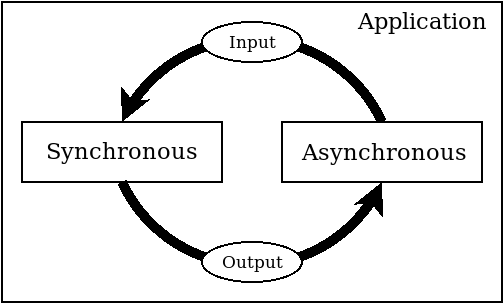
\includegraphics[width=\linewidth]{sync-async}
\caption{ An application in \CEU has a concurrent asynchronous side and a
          predictable synchronous side that receives and reacts to inputs
          atomically.
\label{fig.async}
}
\end{figure}

We propose to extend \CEU with asynchronous ISRs.
However, asynchronous execution confronts the synchronous mindset of \CEU since
the assumption that reactions are atomic no longer holds.
Not only this may lead to race conditions at a fine grain, but may also affect
the ordering of events at a coarse grain: the effect of an earlier event may be
perceived after the effect of a later event.
%
Still, our goal is to preserve the well-behaved interaction between the \CEU
application and the environment even in the presence of asynchronous ISRs.
Figure~\ref{fig.async} adapts the event loop of Figure~\ref{fig.env}, with the
original application represented as the synchronous side and the environment as
the asynchronous side, all inside the same \CEU application.
%
Our idea is to push all subtleties of asynchronous execution into device
drivers, which emit input events to regular synchronous code in \CEU, exactly
as before.

\begin{lstlisting}[
  xleftmargin=1em,
  numbers=left,
  basicstyle=\ttfamily\small,
  float=t,
  caption={Synchronous application that turns the LED on whenever the button
           is pressed and off whenever it is unpressed.},
  label={lst.gpio.sync},
  escapechar=\%,
]
output high/low PIN_13;  // connected to an LED
input  high/low PIN_02;  // connected to a button
#include "gpio.ceu"      // GPIO driver

emit PIN_13(low);
loop do
    var high/low v = await PIN_02;
    emit PIN_13(v);
end
\end{lstlisting}

\begin{lstlisting}[
  xleftmargin=1em,
  numbers=left,
  basicstyle=\ttfamily\small,
  float=t,
  caption={Asynchronous driver for GPIO which, on hardware interrupts, emits an
           input event into a queue.},
  label={lst.gpio.async},
  escapechar=\%,
]
// OUTPUT DRIVER

{ pinMode(13, OUTPUT); }
output (high/low v) PIN_13 do
    { digitalWrite(13, @v); }
end

// INPUT DRIVER

input high/low PIN_02;
{
    pinMode(2, INPUT_PULLUP);
    EICRA |= (1 << ISC00);  // sets INT0
    EIMSK |= (1 << INT0);   // turns on INT0
}
spawn async/isr [INT0_vect] do
    emit PIN_02({digitalRead(2)});
end
\end{lstlisting}

As a first example, Listing~\ref{lst.gpio.sync}~and~\ref{lst.gpio.async} uses
GPIOs to connect a button (pin 02) to an LED (pin 13) via software such that
the LED is on whenever the button is pressed and off whenever it is unpressed.

Listing~\ref{lst.gpio.sync}, the synchronous side, first declares its interface
with the external world and includes the asynchronous side as a driver
(ln~1--3).
It then starts with the LED off (ln~5) and enters a loop (ln~6--9) that,
whenever the button changes (ln~7), toggles the state of the LED with the new
value (ln~8).

Listing~\ref{lst.gpio.async}, the asynchronous side, implements the driver for
the output and input events.
%
An \code{output} implementation (ln~4--6) is similar to a parameterized
subroutine: whenever the application invokes \code{emit}, the output body
executes atomically.
\CEU supports inline C between curly braces (ln~3,5) with interpolation to
evaluate \CEU expressions (e.g., \code{@v}).
This allows drivers to take advantage of existing libraries of embedded
toolchains, such as Arduino.
%
In the example, when the driver is included, it configures pin 13 as output
(ln~3) and sets its new state whenever \code{PIN\_13} is emitted (ln~5).
%
An \code{input} event implementation uses an ISR registered with the
\code{spawn async/isr} primitive (ln~16--18), which is automatically invoked
whenever the associated interrupt occurs (e.g., \code{INT0\_vect}).
%
An ISR in \CEU will typically emit an input event inside its body to awake the
synchronous side (ln~17).
However, although the ISR executes asynchronously when the interrupt occurs,
the \code{emit} goes into a queue (to be discussed) and does not interrupt the
ongoing (suspended) reaction on the synchronous side.
%
In the example, the input driver also configures pin 2 to behave as input and
to generate external interrupts on level transitions (ln~11--15).

The example illustrates the clear separation between the application and the
driver through an event-driven interface that reflects the desired architecture
of Figures~\ref{fig.env}~and~\ref{fig.async}.
%
Now, the whole application is written in \CEU:
    the synchronous side remains well behaved with no low-level calls, and
    the asynchronous side deals with the complexity of device drivers.
%
Nevertheless, drivers are typically write-once components developed by embedded
specialists, which are reused in most applications.
%
Note that each supported architecture requires a mapping between the
\code{async/isr} and the actual interrupt vector table (which we provide
for the \emph{AVR/ATmega} and \emph{ARM/Cortex} microcontrollers).

\begin{lstlisting}[
  xleftmargin=1em,
  numbers=left,
  basicstyle=\ttfamily\small,
  float=t,
  caption={The A/D driver (ln~1--14) is included in the application inside a
           lexically-scoped block (ln~20--24), which turns off all driver
           functionalities automatically on termination.},
  label={lst.adc},
  escapechar=\%,
]
// A/D DRIVER (adc.ceu)

  output int ADC_REQUEST;
  input  int ADC_DONE;

  do finalize with
    {
      ADCSRA &= B01111111;  // disables A/D converter
      ACSR    = B10000000;  // disables comparator
      DIDR0  |= B00111111;  // disables pins
    }
  end
  ...     // driver initialization
  ...     // input / output implementations

// APPLICATION (main.ceu)

  loop do
    var int v;
    do
      #include "adc.ceu" // driver contents above
      emit ADC_REQUEST(A0);
      v = await ADC_DONE;
    end
    ...                  // uses sensor value "v"
    await 1h;
  end
\end{lstlisting}

The example in Listing~\ref{lst.adc} illustrates the use of a lexically-scoped
driver for the A/D converter.
Note that the driver (ln~1--14) and application (ln~16--27) are actually in
separate files.
%
The application is a typical periodic sensor sampling loop, but which
designates an explicit \code{do-end} block (ln~20--24) to include the driver
(ln~21) and use it (ln~22--23).
%
The driver specifies a finalization code (ln~6--12) which executes
unconditionally whenever its enclosing block goes out of scope (ln~24).
The finalize completely disables all A/D functionality to save energy.
%
As discussed in the previous section, the finalizer would also execute if
aborted from a \code{par/or} enclosing the driver.
%
Note that the driver interface (ln~3--4) is visible only inside the block and
thus cannot be inadvertently used outside it.

\subsection{Safe Shared-Memory Concurrency}
\label{sec.ceu.shared}

\begin{figure}[t!]
\begin{minipage}[t]{0.50\linewidth}
\begin{lstlisting}[
  numbers=right,
  xrightmargin=3em,
  basicstyle=\ttfamily\small,
  label={lst.mem.a},
  caption={Shared \code{x}},
  escapechar=\%,
]
input void A;
input void B;
var int x = 1;
par/and do
    await A;
    x = x + 1;
with
    await B;
    x = x * 2;
end
\end{lstlisting}
\end{minipage}%
%
\begin{minipage}[t]{0.50\linewidth}
%\begin{lstlisting}
\begin{lstlisting}[
  xleftmargin=3em,
  basicstyle=\ttfamily\small,
  label={lst.mem.b},
  caption={Shared \code{y}},
  escapechar=\%,
]
input void A;
// (empty line)
var int y = 1;
par/and do
    await A;
    y = y + 1;
with
    await A;
    y = y * 2;
end

\end{lstlisting}
\hskip1.5em
\begin{minipage}[t]{.9\columnwidth}
\end{minipage}%
\end{minipage}%
%\rule{8.4cm}{0.37pt}
\caption{
Accesses to shared \code{x} never concurrent.
Accesses to shared \code{y} are concurrent but still deterministic.},
\label{lst.mem}
\end{figure}

In \CEU, when multiple trails awake in the same reaction, they execute in
lexical order, i.e., in the order they appear in the source code.
%
In Figure~\ref{lst.mem}, both examples define a shared variable (ln~3) and
assign to it in parallel trails (ln~6, 9).
%
In Listing~\ref{lst.mem.a}, the two assignments to \code{x} can only execute in
reactions to different events \code{A} and \code{B} (ln~5,8), which cannot
occur simultaneously in accordance with the synchronous model.
%Hence, for the sequence of events \code{A->B}, \code{x} becomes
%\code{4}~(\code{(1+1)*2}), while for \code{B->A}, \code{x} becomes
%\code{3}~(\code{(1*2)+1}).
In Listing~\ref{lst.mem.b}, the two assignments to \code{y} are simultaneous
because they execute in reaction to the same event \code{A}.
Nevertheless, because \CEU follows lexical order, the execution is still
deterministic, and \code{y} always becomes \code{4} (\code{(1+1)*2}).
%
Even so, \CEU performs (optional) concurrency checks at compile time to detect
conflicting accesses to shared variables:
if a variable is written in a trail segment, then a concurrent trail segment
cannot access that variable~\cite{ceu.sensys13}.
%
%The static checks are optional (or raise warnings) and do not affect the
%semantics of the language.

\begin{lstlisting}[
  xleftmargin=1em,
  numbers=left,
  basicstyle=\ttfamily\small,
  float=t,
  caption={The USART buffer is shared between the ISR and the application,
           resulting in a pontential race condition.
           \emph{(The driver and application code are in separate files.)}},
  label={lst.usart},
]
// USART INTERFACE

input none USART_RX;
var[32*] byte rx_buf;             // `*' = circular

// DRIVER

spawn async/isr [USART_RX_vect] do
    rx_buf = rx_buf .. [{UDR0}];
    emit USART_RX;
end

// APPLICATION

loop do
    await USART_RX;
    var int i;
    loop i in [0 -> $rx_buf[ do   // `$' = length ($)
        // uses rx_buf[i]
    end
    $rx_buf = 0;
end
\end{lstlisting}

The addition of asynchronous ISRs poses real threats concerning race conditions
since they interrupt programs at arbitrary points.
%
Listing~\ref{lst.usart} illustrates a minimum USART application (ln~13--22)
that consumes incoming bytes (ln~18--21) as they arrive (ln~16).
%
The USART API (ln~1--4) exposes an input event to signal incoming data (ln~3)
and a circular buffer to prevent data loss (ln~4).
The buffer is indispensable because the microcontroller may cope with the USART 
speed.
%
The driver ISR (ln~6--11) simply appends incoming bytes to the end of the
buffer (ln~9) and signals the application (ln~10).
%
As a possible race condition, note that the ISR may fire and append a new byte
to the buffer (ln~9) just before the application clears it (ln~21), in which
case the new byte will be lost forever.

\CEU treats an \code{async/isr} as a block of code that runs in parallel with
the rest of the program (hence the required prefix \code{spawn}).
%
This way, it is clear for the compiler that the accesses to \code{rx\_buf} in
Listing~\ref{lst.usart} may lead to a race condition (ln~9,21), and \CEU raises
a compile-time error.
%
The programmer is responsible to protect concurrent memory accesses with
\code{atomic} blocks, which disables interrupts (supposedly) for a short period
of time.

\begin{lstlisting}[
  xleftmargin=1em,
  numbers=left,
  basicstyle=\ttfamily\small,
  float=t,
  caption={The USART driver now exposes a safer (and more friendly) interface
           to the application.
           \emph{(The driver and application code are in separate files.)}},
  label={lst.usart.code},
]
// USART INTERFACE

code Usart_RX (var&[] byte buf, var int n) -> none;

// DRIVER

input none USART_RX;
var[32*] byte rx_buf;

spawn async/isr [USART_RX_vect] do
    rx_buf = rx_buf .. [{UDR0}];
    emit USART_RX;
end

code Usart_RX (var&[] byte buf, var int n) -> none
do
    loop do
        atomic do
            buf = buf..rx_buf;
            $rx_buf = 0;
        end
        if $buf >= n then
            break;
        end
        await USART_RX;
    end
end

// APPLICATION

loop do
    var[255] byte buf;
    await Usart_RX(&buf, 10);
    // uses buf
end
\end{lstlisting}

However, we do not expect that application programmers should be required to
resolve race conditions.
\CEU supports reactive abstractions (similar to coroutines) that help hiding
the concurrency complexity inside the driver.
%
Listing~\ref{lst.usart.code} changes the USART API (ln 1--3) to expose a code
abstraction that expects a reference to a buffer and a number of bytes to
receive.
Now, the application (ln~29--35) invokes the abstraction (ln~33) passing a
local buffer (ln~32).
%
The driver (ln~5--27) now hides the low level interface of the previous example
(ln~7--8) and implements the code abstraction (ln~15--27) that protects the
access to the shared buffer with an \code{atomic} block (ln~18--21).
%
The abstraction copies the driver buffer into the application buffer (ln~19)
up to the requested number of bytes (ln~22).
%
On the one hand the extra copying incurs a memory and runtime overhead, but on
the other hand it prevents race conditions with the ISR.

Support for ISRs in the same language and memory space of the application
allows programmers to choose between efficiency and safety during development
by providing multiple interfaces with different levels of abstraction.

\subsection{Energy-Efficient Runtime}
\label{sec.energy}

\begin{lstlisting}[
  xleftmargin=1em,
  numbers=left,
  basicstyle=\ttfamily\small,
  float=t,
  caption={Overall runtime architecture of \CEU with an input queue (ln~1),
           event loop (ln~4--11), synchronous execution (ln~7), and standby
           mode (ln~9).},
  label={lst.env},
]
evt_t queue[MAX];           // input queue
void main () {
  ceu_start();              // "boot reaction"
  while (1) {
    evt_t evt;
    if (ceu_input(&evt)) {  // query input queue
      ceu_sync(&evt);       // execute synchronous
    } else {
      ceu_pm_sleep();       // nothing to execute
    }
  }
}
\end{lstlisting}

Our runtime implements the event loop proposed in Figure~\ref{fig.async}, which
alternates between synchronous, well-behaved execution, and asynchronous,
unpredictable ISRs.
%
Since the language now has full control over the event loop and only executes
from interrupts, it is possible for the runtime to enter in sleep mode
automatically to save energy.

Listing~\ref{lst.env} is a realization of this architecture:
%
The runtime defines an input queue (ln~1) in which ISRs enqueue new events
(e.g., Listing~\ref{lst.usart.code}, ln~12).
%
In the \code{main} function, we first generate the \emph{boot reaction} (ln~3),
which starts the program, spawns the ISRs, and reaches the first \code{await}
statements in the multiple lines of code.
%
Then, the runtime enters an infinite loop (ln~4--11) that queries the input
queue (ln~6) to awake the program (ln~7).
%
Note that ISRs execute asynchronously with the loop, but they typically only
emit an input event into the queue which will be queried in a subsequent
iteration.
%
Note also that if the queue is empty, the runtime enters in sleep mode to save
energy (ln~9), and will only awake on a new hardware interrupt.

Microcontrollers typically support multiple levels of sleep mode, each
progressively saves more energy at the expense of keeping less functionality
active.
%
As an example, the least efficient mode of the \emph{ATmega328P} allows for
timer interrupts since it keeps its internal clock active, while the most
efficient mode turns off all peripherals and can only awake from external
interrupts.

Our runtime supports three compile-time configurations for \code{ceu\_pm\_sleep}
(ln~9):
%
The first configuration is a \emph{nop} which simply keeps the event loop
running all the time without ever sleeping.
This configuration is useful when introducing new platforms.
%
The second configuration chooses a (inefficient) sleep mode that keeps all
peripherals active.
Although this configuration is not the most energy efficient, at least, it
requires no extra assistance from the drivers.
%
The third configuration keeps a bit vector of the active drivers during runtime
and chooses the most efficient mode, querying this vector every time
\code{ceu\_pm\_sleep} is called.

\begin{lstlisting}[
  xleftmargin=1em,
  numbers=left,
  basicstyle=\ttfamily\small,
  float=t,
  caption={Interaction between the power manager, USART driver, and application
           (each code is actually in a separate file).},
  label={lst.pm},
  escapechar=\%,
]
// POWER MANAGER (in C)

enum {
    CEU_PM_ADC,
    CEU_PM_TIMER1,
    CEU_PM_USART,
    ...
};

void ceu_pm_sleep (void) {
    if (ceu_pm_get(CEU_PM_USART) || ...) {
        sleep_mode_1(...);
    } else if (ceu_pm_get(CEU_PM_ADC)) {
        sleep_mode_2(...);
    } else {
        sleep_mode_3(...);
    }
}

// USART DRIVER (in Ceu)

code Usart_RX (var&[] byte buf, var int n) -> none
do
    {ceu_pm_set(CEU_PM_USART, 1);}
    do finalize with
        {ceu_pm_set(CEU_PM_USART, 0);}
    end
    ...   // same as in Listing 7
end

// APPLICATION (in Ceu)

input high/low PIN_02;      // connected to a button
loop do
    par/or do
        await PIN_02;
    with
        var[255] byte buf;
        await Usart_RX(&buf, 10);
        // uses buf
    end
    await PIN_02;
end
\end{lstlisting}

The third configuration achieves optimal efficiency but requires a tight
interaction between the drivers and the power management runtime.
%
Listing~\ref{lst.pm} unveils the power manager (ln~1--18), the modified USART
driver (ln~20--29), and an illustrative application (ln~31--43).
%
The application is a loop that awaits in parallel for a button press (ln~36) or
receiving 10 bytes (ln~39).
Let's call this initial state \code{STATE-A}.
The \code{par/or} terminates when either of them occurs, going to the next line
that awaits another button click (ln~42).
Let's call this other state \code{STATE-B}.
After the button click, the program loops back to \code{STATE-A}.
%
While in \code{STATE-A}, the program can awake from USART and external
interrupts, which means that the power manager should choose a sleep mode in
which the USART remains operational.
%
While in \code{STATE-B}, only external interrupts should awake the program,
which means that the power manager may use the most efficient sleep mode.
%
The power manager enumerates all microcontroller's peripherals (ln~3--8) and,
before sleeping, queries their states (ln~11,13) to choose the most appropriate
sleep mode (ln~12,14,16).
%
The USART driver needs to be extended with calls to enable and disable the
USART state inside the power manager: just before awaiting, the driver enables
the USART (ln~24) and creates a finalization block to unregister it on
termination (ln~25--27).
Termination may occur either directly after receiving the requested number of
bytes, or indirectly if the \code{par/or} in the application terminates on a
button click (ln~36).

Note that applications need not to be explicit about energy management to take
advantage of sleep modes.
All happens automatically because of the synchronous-reactive execution model
and energy-aware runtime of \CEU.

\section{Related Work}

- TinyOS
    - async, race condition avoidance
        - nesc manual
    - ICEM, standby
        - icem paper

- CRP

- finalize
- structured programming
    - lexical scoping vs manual
    - no turn off

- citar ICEM o mais cedo nas duas ocasioes (async, energy)
- citar TOS/ICEM na introducao como maior influencia
    - ja no abstract?

- falar que async/isr nao contem nada de Ceu, apenas shared memory e nocao de estar em paralelo
    - compartilhamento de memoria
        - velocidade
    - ajuda do compilador p/ detectar acesso concorrente

- finite is can be still much greater than 0 (order of milliseconds)
    - which is a lot of time

%% Acknowledgments
\begin{acks}                            %% acks environment is optional
                                        %% contents suppressed with 'anonymous'
  %% Commands \grantsponsor{<sponsorID>}{<name>}{<url>} and
  %% \grantnum[<url>]{<sponsorID>}{<number>} should be used to
  %% acknowledge financial support and will be used by metadata
  %% extraction tools.
  This material is based upon work supported by the
  \grantsponsor{GS100000001}{National Science
    Foundation}{http://dx.doi.org/10.13039/100000001} under Grant
  No.~\grantnum{GS100000001}{nnnnnnn} and Grant
  No.~\grantnum{GS100000001}{mmmmmmm}.  Any opinions, findings, and
  conclusions or recommendations expressed in this material are those
  of the author and do not necessarily reflect the views of the
  National Science Foundation.
\end{acks}


%% Bibliography
\bibliography{my,other}


%% Appendix
\appendix
\section{Appendix}

Text of appendix \ldots

\end{document}
